\PassOptionsToPackage{unicode=true}{hyperref} % options for packages loaded elsewhere
\PassOptionsToPackage{hyphens}{url}
%
\documentclass[]{article}
\usepackage{lmodern}
\usepackage{amssymb,amsmath}
\usepackage{ifxetex,ifluatex}
\usepackage{fixltx2e} % provides \textsubscript
\ifnum 0\ifxetex 1\fi\ifluatex 1\fi=0 % if pdftex
  \usepackage[T1]{fontenc}
  \usepackage[utf8]{inputenc}
  \usepackage{textcomp} % provides euro and other symbols
\else % if luatex or xelatex
  \usepackage{unicode-math}
  \defaultfontfeatures{Ligatures=TeX,Scale=MatchLowercase}
\fi
% use upquote if available, for straight quotes in verbatim environments
\IfFileExists{upquote.sty}{\usepackage{upquote}}{}
% use microtype if available
\IfFileExists{microtype.sty}{%
\usepackage[]{microtype}
\UseMicrotypeSet[protrusion]{basicmath} % disable protrusion for tt fonts
}{}
\IfFileExists{parskip.sty}{%
\usepackage{parskip}
}{% else
\setlength{\parindent}{0pt}
\setlength{\parskip}{6pt plus 2pt minus 1pt}
}
\usepackage{hyperref}
\hypersetup{
            pdftitle={Assignment 5: Data Visualization},
            pdfauthor={Rachel Gonsenhauser},
            pdfborder={0 0 0},
            breaklinks=true}
\urlstyle{same}  % don't use monospace font for urls
\usepackage[margin=2.54cm]{geometry}
\usepackage{color}
\usepackage{fancyvrb}
\newcommand{\VerbBar}{|}
\newcommand{\VERB}{\Verb[commandchars=\\\{\}]}
\DefineVerbatimEnvironment{Highlighting}{Verbatim}{commandchars=\\\{\}}
% Add ',fontsize=\small' for more characters per line
\usepackage{framed}
\definecolor{shadecolor}{RGB}{248,248,248}
\newenvironment{Shaded}{\begin{snugshade}}{\end{snugshade}}
\newcommand{\AlertTok}[1]{\textcolor[rgb]{0.94,0.16,0.16}{#1}}
\newcommand{\AnnotationTok}[1]{\textcolor[rgb]{0.56,0.35,0.01}{\textbf{\textit{#1}}}}
\newcommand{\AttributeTok}[1]{\textcolor[rgb]{0.77,0.63,0.00}{#1}}
\newcommand{\BaseNTok}[1]{\textcolor[rgb]{0.00,0.00,0.81}{#1}}
\newcommand{\BuiltInTok}[1]{#1}
\newcommand{\CharTok}[1]{\textcolor[rgb]{0.31,0.60,0.02}{#1}}
\newcommand{\CommentTok}[1]{\textcolor[rgb]{0.56,0.35,0.01}{\textit{#1}}}
\newcommand{\CommentVarTok}[1]{\textcolor[rgb]{0.56,0.35,0.01}{\textbf{\textit{#1}}}}
\newcommand{\ConstantTok}[1]{\textcolor[rgb]{0.00,0.00,0.00}{#1}}
\newcommand{\ControlFlowTok}[1]{\textcolor[rgb]{0.13,0.29,0.53}{\textbf{#1}}}
\newcommand{\DataTypeTok}[1]{\textcolor[rgb]{0.13,0.29,0.53}{#1}}
\newcommand{\DecValTok}[1]{\textcolor[rgb]{0.00,0.00,0.81}{#1}}
\newcommand{\DocumentationTok}[1]{\textcolor[rgb]{0.56,0.35,0.01}{\textbf{\textit{#1}}}}
\newcommand{\ErrorTok}[1]{\textcolor[rgb]{0.64,0.00,0.00}{\textbf{#1}}}
\newcommand{\ExtensionTok}[1]{#1}
\newcommand{\FloatTok}[1]{\textcolor[rgb]{0.00,0.00,0.81}{#1}}
\newcommand{\FunctionTok}[1]{\textcolor[rgb]{0.00,0.00,0.00}{#1}}
\newcommand{\ImportTok}[1]{#1}
\newcommand{\InformationTok}[1]{\textcolor[rgb]{0.56,0.35,0.01}{\textbf{\textit{#1}}}}
\newcommand{\KeywordTok}[1]{\textcolor[rgb]{0.13,0.29,0.53}{\textbf{#1}}}
\newcommand{\NormalTok}[1]{#1}
\newcommand{\OperatorTok}[1]{\textcolor[rgb]{0.81,0.36,0.00}{\textbf{#1}}}
\newcommand{\OtherTok}[1]{\textcolor[rgb]{0.56,0.35,0.01}{#1}}
\newcommand{\PreprocessorTok}[1]{\textcolor[rgb]{0.56,0.35,0.01}{\textit{#1}}}
\newcommand{\RegionMarkerTok}[1]{#1}
\newcommand{\SpecialCharTok}[1]{\textcolor[rgb]{0.00,0.00,0.00}{#1}}
\newcommand{\SpecialStringTok}[1]{\textcolor[rgb]{0.31,0.60,0.02}{#1}}
\newcommand{\StringTok}[1]{\textcolor[rgb]{0.31,0.60,0.02}{#1}}
\newcommand{\VariableTok}[1]{\textcolor[rgb]{0.00,0.00,0.00}{#1}}
\newcommand{\VerbatimStringTok}[1]{\textcolor[rgb]{0.31,0.60,0.02}{#1}}
\newcommand{\WarningTok}[1]{\textcolor[rgb]{0.56,0.35,0.01}{\textbf{\textit{#1}}}}
\usepackage{graphicx,grffile}
\makeatletter
\def\maxwidth{\ifdim\Gin@nat@width>\linewidth\linewidth\else\Gin@nat@width\fi}
\def\maxheight{\ifdim\Gin@nat@height>\textheight\textheight\else\Gin@nat@height\fi}
\makeatother
% Scale images if necessary, so that they will not overflow the page
% margins by default, and it is still possible to overwrite the defaults
% using explicit options in \includegraphics[width, height, ...]{}
\setkeys{Gin}{width=\maxwidth,height=\maxheight,keepaspectratio}
\setlength{\emergencystretch}{3em}  % prevent overfull lines
\providecommand{\tightlist}{%
  \setlength{\itemsep}{0pt}\setlength{\parskip}{0pt}}
\setcounter{secnumdepth}{0}
% Redefines (sub)paragraphs to behave more like sections
\ifx\paragraph\undefined\else
\let\oldparagraph\paragraph
\renewcommand{\paragraph}[1]{\oldparagraph{#1}\mbox{}}
\fi
\ifx\subparagraph\undefined\else
\let\oldsubparagraph\subparagraph
\renewcommand{\subparagraph}[1]{\oldsubparagraph{#1}\mbox{}}
\fi

% set default figure placement to htbp
\makeatletter
\def\fps@figure{htbp}
\makeatother


\title{Assignment 5: Data Visualization}
\author{Rachel Gonsenhauser}
\date{}

\begin{document}
\maketitle

\hypertarget{overview}{%
\subsection{OVERVIEW}\label{overview}}

This exercise accompanies the lessons in Environmental Data Analytics on
Data Visualization

\hypertarget{directions}{%
\subsection{Directions}\label{directions}}

\begin{enumerate}
\def\labelenumi{\arabic{enumi}.}
\tightlist
\item
  Change ``Student Name'' on line 3 (above) with your name.
\item
  Work through the steps, \textbf{creating code and output} that fulfill
  each instruction.
\item
  Be sure to \textbf{answer the questions} in this assignment document.
\item
  When you have completed the assignment, \textbf{Knit} the text and
  code into a single PDF file.
\item
  After Knitting, submit the completed exercise (PDF file) to the
  dropbox in Sakai. Add your last name into the file name (e.g.,
  ``Salk\_A05\_DataVisualization.Rmd'') prior to submission.
\end{enumerate}

The completed exercise is due on Tuesday, February 11 at 1:00 pm.

\hypertarget{set-up-your-session}{%
\subsection{Set up your session}\label{set-up-your-session}}

\begin{enumerate}
\def\labelenumi{\arabic{enumi}.}
\item
  Set up your session. Verify your working directory and load the
  tidyverse and cowplot packages. Upload the NTL-LTER processed data
  files for nutrients and chemistry/physics for Peter and Paul Lakes
  (tidy and gathered) and the processed data file for the Niwot Ridge
  litter dataset.
\item
  Make sure R is reading dates as date format; if not change the format
  to date.
\end{enumerate}

\begin{Shaded}
\begin{Highlighting}[]
\CommentTok{#1}
\KeywordTok{getwd}\NormalTok{()}
\end{Highlighting}
\end{Shaded}

\begin{verbatim}
## [1] "/Users/rachelgonsenhauser/Documents/Environmental_Data_Analytics_2020"
\end{verbatim}

\begin{Shaded}
\begin{Highlighting}[]
\KeywordTok{library}\NormalTok{(tidyverse)}
\end{Highlighting}
\end{Shaded}

\begin{verbatim}
## -- Attaching packages ---------------------------------------------------------- tidyverse 1.3.0 --
\end{verbatim}

\begin{verbatim}
## v ggplot2 3.2.1     v purrr   0.3.3
## v tibble  2.1.3     v dplyr   0.8.3
## v tidyr   1.0.0     v stringr 1.4.0
## v readr   1.3.1     v forcats 0.4.0
\end{verbatim}

\begin{verbatim}
## -- Conflicts ------------------------------------------------------------- tidyverse_conflicts() --
## x dplyr::filter() masks stats::filter()
## x dplyr::lag()    masks stats::lag()
\end{verbatim}

\begin{Shaded}
\begin{Highlighting}[]
\KeywordTok{library}\NormalTok{(cowplot)}
\end{Highlighting}
\end{Shaded}

\begin{verbatim}
## 
## ********************************************************
\end{verbatim}

\begin{verbatim}
## Note: As of version 1.0.0, cowplot does not change the
\end{verbatim}

\begin{verbatim}
##   default ggplot2 theme anymore. To recover the previous
\end{verbatim}

\begin{verbatim}
##   behavior, execute:
##   theme_set(theme_cowplot())
\end{verbatim}

\begin{verbatim}
## ********************************************************
\end{verbatim}

\begin{Shaded}
\begin{Highlighting}[]
\NormalTok{PeterPaul.chem.nutrients <-}
\StringTok{  }\KeywordTok{read.csv}\NormalTok{(}\StringTok{"./Data/Processed/NTL-LTER_Lake_Chemistry_Nutrients_PeterPaul_Processed.csv"}\NormalTok{)}
\NormalTok{PeterPaul.chem.nutrients.gathered <-}\StringTok{ }
\StringTok{  }\KeywordTok{read.csv}\NormalTok{(}\StringTok{"./Data/Processed/NTL-LTER_Lake_Nutrients_PeterPaulGathered_Processed.csv"}\NormalTok{)}
\NormalTok{Litter <-}\StringTok{ }
\StringTok{  }\KeywordTok{read.csv}\NormalTok{(}\StringTok{"./Data/Processed/NEON_NIWO_Litter_mass_trap_Processed.csv"}\NormalTok{)}

\CommentTok{#2}
\KeywordTok{class}\NormalTok{(PeterPaul.chem.nutrients}\OperatorTok{$}\NormalTok{sampledate)}
\end{Highlighting}
\end{Shaded}

\begin{verbatim}
## [1] "factor"
\end{verbatim}

\begin{Shaded}
\begin{Highlighting}[]
\KeywordTok{class}\NormalTok{(PeterPaul.chem.nutrients.gathered}\OperatorTok{$}\NormalTok{sampledate)}
\end{Highlighting}
\end{Shaded}

\begin{verbatim}
## [1] "factor"
\end{verbatim}

\begin{Shaded}
\begin{Highlighting}[]
\KeywordTok{class}\NormalTok{(Litter}\OperatorTok{$}\NormalTok{collectDate)}
\end{Highlighting}
\end{Shaded}

\begin{verbatim}
## [1] "factor"
\end{verbatim}

\begin{Shaded}
\begin{Highlighting}[]
\NormalTok{PeterPaul.chem.nutrients}\OperatorTok{$}\NormalTok{sampledate <-}\StringTok{ }
\StringTok{  }\KeywordTok{as.Date}\NormalTok{(PeterPaul.chem.nutrients}\OperatorTok{$}\NormalTok{sampledate, }
          \DataTypeTok{format =} \StringTok{"%Y-%m-%d"}\NormalTok{)}
\NormalTok{PeterPaul.chem.nutrients.gathered}\OperatorTok{$}\NormalTok{sampledate <-}
\StringTok{  }\KeywordTok{as.Date}\NormalTok{(PeterPaul.chem.nutrients.gathered}\OperatorTok{$}\NormalTok{sampledate, }
          \DataTypeTok{format =} \StringTok{"%Y-%m-%d"}\NormalTok{)}
\NormalTok{Litter}\OperatorTok{$}\NormalTok{collectDate <-}\StringTok{ }
\StringTok{  }\KeywordTok{as.Date}\NormalTok{(Litter}\OperatorTok{$}\NormalTok{collectDate, }\DataTypeTok{format =} \StringTok{"%Y-%m-%d"}\NormalTok{)}

\KeywordTok{class}\NormalTok{(PeterPaul.chem.nutrients}\OperatorTok{$}\NormalTok{sampledate)}
\end{Highlighting}
\end{Shaded}

\begin{verbatim}
## [1] "Date"
\end{verbatim}

\begin{Shaded}
\begin{Highlighting}[]
\KeywordTok{class}\NormalTok{(PeterPaul.chem.nutrients.gathered}\OperatorTok{$}\NormalTok{sampledate)}
\end{Highlighting}
\end{Shaded}

\begin{verbatim}
## [1] "Date"
\end{verbatim}

\begin{Shaded}
\begin{Highlighting}[]
\KeywordTok{class}\NormalTok{(Litter}\OperatorTok{$}\NormalTok{collectDate)}
\end{Highlighting}
\end{Shaded}

\begin{verbatim}
## [1] "Date"
\end{verbatim}

\hypertarget{define-your-theme}{%
\subsection{Define your theme}\label{define-your-theme}}

\begin{enumerate}
\def\labelenumi{\arabic{enumi}.}
\setcounter{enumi}{2}
\tightlist
\item
  Build a theme and set it as your default theme.
\end{enumerate}

\begin{Shaded}
\begin{Highlighting}[]
\NormalTok{mytheme <-}\StringTok{ }\KeywordTok{theme_classic}\NormalTok{(}\DataTypeTok{base_size =} \DecValTok{10}\NormalTok{) }\OperatorTok{+}
\StringTok{  }\KeywordTok{theme}\NormalTok{(}\DataTypeTok{axis.text =} \KeywordTok{element_text}\NormalTok{(}\DataTypeTok{color =} \StringTok{"black"}\NormalTok{), }
        \DataTypeTok{legend.position =} \StringTok{"bottom"}\NormalTok{)}

\KeywordTok{theme_set}\NormalTok{(mytheme)}
\end{Highlighting}
\end{Shaded}

\hypertarget{create-graphs}{%
\subsection{Create graphs}\label{create-graphs}}

For numbers 4-7, create ggplot graphs and adjust aesthetics to follow
best practices for data visualization. Ensure your theme, color
palettes, axes, and additional aesthetics are edited accordingly.

\begin{enumerate}
\def\labelenumi{\arabic{enumi}.}
\setcounter{enumi}{3}
\tightlist
\item
  {[}NTL-LTER{]} Plot total phosphorus by phosphate, with separate
  aesthetics for Peter and Paul lakes. Add a line of best fit and color
  it black. Adjust your axes to hide extreme values.
\end{enumerate}

\begin{Shaded}
\begin{Highlighting}[]
\KeywordTok{library}\NormalTok{(viridis)}
\end{Highlighting}
\end{Shaded}

\begin{verbatim}
## Loading required package: viridisLite
\end{verbatim}

\begin{Shaded}
\begin{Highlighting}[]
\KeywordTok{library}\NormalTok{(RColorBrewer)}
\KeywordTok{library}\NormalTok{(colormap)}

\NormalTok{Pplot1 <-}\StringTok{ }\KeywordTok{ggplot}\NormalTok{(PeterPaul.chem.nutrients) }\OperatorTok{+}
\StringTok{  }\KeywordTok{geom_point}\NormalTok{(}\KeywordTok{aes}\NormalTok{(}\DataTypeTok{x =}\NormalTok{ po4, }\DataTypeTok{y =}\NormalTok{ tp_ug, }\DataTypeTok{color =}\NormalTok{ lakename)) }\OperatorTok{+}
\StringTok{    }\KeywordTok{geom_smooth}\NormalTok{(}\KeywordTok{aes}\NormalTok{(}\DataTypeTok{x =}\NormalTok{po4, }\DataTypeTok{y =}\NormalTok{ tp_ug), }\DataTypeTok{color =} \StringTok{"black"}\NormalTok{,}
                \DataTypeTok{method =}\NormalTok{ lm, }\DataTypeTok{se =} \OtherTok{FALSE}\NormalTok{) }\OperatorTok{+}
\StringTok{   }\KeywordTok{labs}\NormalTok{(}\DataTypeTok{x =} \KeywordTok{expression}\NormalTok{(PO4 }\OperatorTok{~}\StringTok{ }\NormalTok{(mu}\OperatorTok{*}\NormalTok{g }\OperatorTok{/}\StringTok{ }\NormalTok{L)), }\DataTypeTok{y =} \KeywordTok{expression}\NormalTok{(TP }\OperatorTok{~}\StringTok{ }\NormalTok{(mu}\OperatorTok{*}\NormalTok{g }\OperatorTok{/}\StringTok{ }\NormalTok{L)),}
       \DataTypeTok{color =} \StringTok{""}\NormalTok{) }\OperatorTok{+}
\StringTok{  }\KeywordTok{scale_color_brewer}\NormalTok{(}\DataTypeTok{palette =} \StringTok{"Set1"}\NormalTok{) }\OperatorTok{+}
\StringTok{  }\KeywordTok{xlim}\NormalTok{(}\DecValTok{0}\NormalTok{, }\DecValTok{50}\NormalTok{) }\OperatorTok{+}
\StringTok{  }\KeywordTok{ylim}\NormalTok{(}\DecValTok{0}\NormalTok{, }\DecValTok{200}\NormalTok{)}
\KeywordTok{print}\NormalTok{(Pplot1)}
\end{Highlighting}
\end{Shaded}

\begin{verbatim}
## Warning: Removed 21948 rows containing non-finite values (stat_smooth).
\end{verbatim}

\begin{verbatim}
## Warning: Removed 21948 rows containing missing values (geom_point).
\end{verbatim}

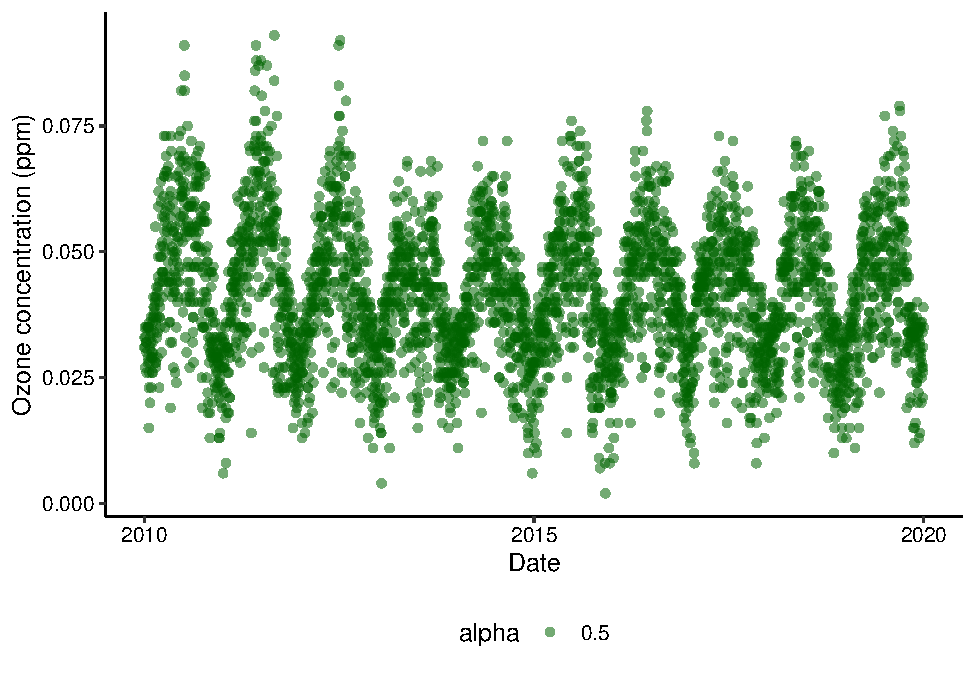
\includegraphics{A05_DataVisualization_Gonsenhauser_files/figure-latex/unnamed-chunk-3-1.pdf}

\begin{enumerate}
\def\labelenumi{\arabic{enumi}.}
\setcounter{enumi}{4}
\tightlist
\item
  {[}NTL-LTER{]} Make three separate boxplots of (a) temperature, (b)
  TP, and (c) TN, with month as the x axis and lake as a color
  aesthetic. Then, create a cowplot that combines the three graphs. Make
  sure that only one legend is present and that graph axes are aligned.
\end{enumerate}

\begin{Shaded}
\begin{Highlighting}[]
\NormalTok{TempPlot <-}\StringTok{ }\KeywordTok{ggplot}\NormalTok{(PeterPaul.chem.nutrients) }\OperatorTok{+}
\StringTok{  }\KeywordTok{geom_boxplot}\NormalTok{(}\KeywordTok{aes}\NormalTok{(}\DataTypeTok{x =} \KeywordTok{as.factor}\NormalTok{(month), }\DataTypeTok{y =}\NormalTok{ temperature_C, }\DataTypeTok{color =}\NormalTok{ lakename)) }\OperatorTok{+}
\StringTok{   }\KeywordTok{labs}\NormalTok{(}\DataTypeTok{x =} \KeywordTok{expression}\NormalTok{(month), }\DataTypeTok{y =} \KeywordTok{expression}\NormalTok{(temperature }\OperatorTok{~}\StringTok{ }\NormalTok{(C)),}
       \DataTypeTok{color =} \StringTok{""}\NormalTok{) }\OperatorTok{+}
\StringTok{  }\KeywordTok{scale_color_brewer}\NormalTok{(}\DataTypeTok{palette =} \StringTok{"Set1"}\NormalTok{) }
\KeywordTok{print}\NormalTok{(TempPlot)}
\end{Highlighting}
\end{Shaded}

\begin{verbatim}
## Warning: Removed 3566 rows containing non-finite values (stat_boxplot).
\end{verbatim}

\includegraphics{A05_DataVisualization_Gonsenhauser_files/figure-latex/unnamed-chunk-4-1.pdf}

\begin{Shaded}
\begin{Highlighting}[]
\NormalTok{TPPlot <-}\StringTok{ }\KeywordTok{ggplot}\NormalTok{(PeterPaul.chem.nutrients) }\OperatorTok{+}
\StringTok{  }\KeywordTok{geom_boxplot}\NormalTok{(}\KeywordTok{aes}\NormalTok{(}\DataTypeTok{x =} \KeywordTok{as.factor}\NormalTok{(month), }\DataTypeTok{y =}\NormalTok{ tp_ug, }\DataTypeTok{color =}\NormalTok{ lakename)) }\OperatorTok{+}
\StringTok{   }\KeywordTok{labs}\NormalTok{(}\DataTypeTok{x =} \KeywordTok{expression}\NormalTok{(month), }\DataTypeTok{y =} \KeywordTok{expression}\NormalTok{(TP }\OperatorTok{~}\StringTok{ }\NormalTok{(mu}\OperatorTok{*}\NormalTok{g }\OperatorTok{/}\StringTok{ }\NormalTok{L)),}
       \DataTypeTok{color =} \StringTok{""}\NormalTok{) }\OperatorTok{+}
\StringTok{  }\KeywordTok{scale_color_brewer}\NormalTok{(}\DataTypeTok{palette =} \StringTok{"Set1"}\NormalTok{) }
\KeywordTok{print}\NormalTok{(TPPlot)}
\end{Highlighting}
\end{Shaded}

\begin{verbatim}
## Warning: Removed 20729 rows containing non-finite values (stat_boxplot).
\end{verbatim}

\includegraphics{A05_DataVisualization_Gonsenhauser_files/figure-latex/unnamed-chunk-4-2.pdf}

\begin{Shaded}
\begin{Highlighting}[]
\NormalTok{TNPlot <-}\StringTok{ }\KeywordTok{ggplot}\NormalTok{(PeterPaul.chem.nutrients) }\OperatorTok{+}
\StringTok{  }\KeywordTok{geom_boxplot}\NormalTok{(}\KeywordTok{aes}\NormalTok{(}\DataTypeTok{x =} \KeywordTok{as.factor}\NormalTok{(month), }\DataTypeTok{y =}\NormalTok{ tn_ug, }\DataTypeTok{color =}\NormalTok{ lakename)) }\OperatorTok{+}
\StringTok{   }\KeywordTok{labs}\NormalTok{(}\DataTypeTok{x =} \KeywordTok{expression}\NormalTok{(month), }\DataTypeTok{y =} \KeywordTok{expression}\NormalTok{(TN }\OperatorTok{~}\StringTok{ }\NormalTok{(mu}\OperatorTok{*}\NormalTok{g }\OperatorTok{/}\StringTok{ }\NormalTok{L)),}
       \DataTypeTok{color =} \StringTok{""}\NormalTok{) }\OperatorTok{+}
\StringTok{  }\KeywordTok{scale_color_brewer}\NormalTok{(}\DataTypeTok{palette =} \StringTok{"Set1"}\NormalTok{) }
\KeywordTok{print}\NormalTok{(TNPlot)}
\end{Highlighting}
\end{Shaded}

\begin{verbatim}
## Warning: Removed 21583 rows containing non-finite values (stat_boxplot).
\end{verbatim}

\includegraphics{A05_DataVisualization_Gonsenhauser_files/figure-latex/unnamed-chunk-4-3.pdf}

\begin{Shaded}
\begin{Highlighting}[]
\KeywordTok{library}\NormalTok{(cowplot)}
\KeywordTok{plot_grid}\NormalTok{((TempPlot }\OperatorTok{+}\StringTok{ }\KeywordTok{theme}\NormalTok{(}\DataTypeTok{legend.position =} \StringTok{"none"}\NormalTok{)), (TPPlot }\OperatorTok{+}\StringTok{ }\KeywordTok{theme}\NormalTok{(}\DataTypeTok{legend.position =} \StringTok{"none"}\NormalTok{)), (TNPlot }\OperatorTok{+}\StringTok{ }\KeywordTok{theme}\NormalTok{(}\DataTypeTok{legend.position =} \StringTok{"bottom"}\NormalTok{)), }\DataTypeTok{nrow =} \DecValTok{3}\NormalTok{, }\DataTypeTok{rel_heights =} \KeywordTok{c}\NormalTok{(}\DecValTok{1}\NormalTok{, }\DecValTok{1}\NormalTok{, }\FloatTok{1.25}\NormalTok{), }\DataTypeTok{align =} \StringTok{'hv'}\NormalTok{)}
\end{Highlighting}
\end{Shaded}

\begin{verbatim}
## Warning: Removed 3566 rows containing non-finite values (stat_boxplot).
\end{verbatim}

\begin{verbatim}
## Warning: Removed 20729 rows containing non-finite values (stat_boxplot).
\end{verbatim}

\begin{verbatim}
## Warning: Removed 21583 rows containing non-finite values (stat_boxplot).
\end{verbatim}

\begin{verbatim}
## Warning: Graphs cannot be horizontally aligned unless the axis parameter is set.
## Placing graphs unaligned.
\end{verbatim}

\includegraphics{A05_DataVisualization_Gonsenhauser_files/figure-latex/unnamed-chunk-4-4.pdf}

\begin{Shaded}
\begin{Highlighting}[]
\NormalTok{print}
\end{Highlighting}
\end{Shaded}

\begin{verbatim}
## function (x, ...) 
## UseMethod("print")
## <bytecode: 0x7f9639152448>
## <environment: namespace:base>
\end{verbatim}

Question: What do you observe about the variables of interest over
seasons and between lakes?

\begin{quote}
Answer: Temperature increases during the summer and early fall months.
There is not a marked difference in temperature between the two lakes.
Total phosphorouus does not appear to have much seasonal variability and
there are many outliers (particularly higher value outliers) for
observations in both lakes. Peter Lake consistently has higher median
values of total phosphorous across seasons. Total nitrogen, like total
phosphorous, does not appear to have much seasonal variability and there
are many upper-value outliers. Peter Lake, again, has higher median
values of total nitrogen across seasons.
\end{quote}

\begin{enumerate}
\def\labelenumi{\arabic{enumi}.}
\setcounter{enumi}{5}
\tightlist
\item
  {[}Niwot Ridge{]} Plot a subset of the litter dataset by displaying
  only the ``Needles'' functional group. Plot the dry mass of needle
  litter by date and separate by NLCD class with a color aesthetic. (no
  need to adjust the name of each land use)
\end{enumerate}

\begin{Shaded}
\begin{Highlighting}[]
\NormalTok{Needles <-}\StringTok{  }\KeywordTok{filter}\NormalTok{(Litter, functionalGroup }\OperatorTok
\StringTok{           }\KeywordTok{c}\NormalTok{(}\StringTok{"Needles"}\NormalTok{))}

\NormalTok{NeedlesPlot <-}\StringTok{ }\KeywordTok{ggplot}\NormalTok{(Needles) }\OperatorTok{+}
\StringTok{  }\KeywordTok{geom_point}\NormalTok{(}\KeywordTok{aes}\NormalTok{(}\DataTypeTok{x =}\NormalTok{ collectDate, }\DataTypeTok{y =}\NormalTok{ dryMass, }\DataTypeTok{color =}\NormalTok{nlcdClass)) }\OperatorTok{+}
\StringTok{  }\KeywordTok{labs}\NormalTok{(}\DataTypeTok{x =} \KeywordTok{expression}\NormalTok{(}\StringTok{"collection date"}\NormalTok{), }\DataTypeTok{y =} \KeywordTok{expression}\NormalTok{(}\StringTok{"dry mass (grams)"}\NormalTok{),}
       \DataTypeTok{color =} \StringTok{""}\NormalTok{) }\OperatorTok{+}
\StringTok{  }\KeywordTok{scale_color_brewer}\NormalTok{(}\DataTypeTok{palette =} \StringTok{"Set1"}\NormalTok{)}
\KeywordTok{print}\NormalTok{(NeedlesPlot)}
\end{Highlighting}
\end{Shaded}

\includegraphics{A05_DataVisualization_Gonsenhauser_files/figure-latex/unnamed-chunk-5-1.pdf}

\begin{enumerate}
\def\labelenumi{\arabic{enumi}.}
\setcounter{enumi}{6}
\tightlist
\item
  {[}Niwot Ridge{]} Now, plot the same plot but with NLCD classes
  separated into three facets rather than separated by color.
\end{enumerate}

\begin{Shaded}
\begin{Highlighting}[]
\NormalTok{NeedlesPlot2 <-}\StringTok{ }\KeywordTok{ggplot}\NormalTok{(Needles) }\OperatorTok{+}
\StringTok{  }\KeywordTok{geom_point}\NormalTok{(}\KeywordTok{aes}\NormalTok{(}\DataTypeTok{x =}\NormalTok{ collectDate, }\DataTypeTok{y =}\NormalTok{ dryMass)) }\OperatorTok{+}
\StringTok{  }\KeywordTok{facet_wrap}\NormalTok{(}\KeywordTok{vars}\NormalTok{(nlcdClass), }\DataTypeTok{nrow =} \DecValTok{3}\NormalTok{) }\OperatorTok{+}
\StringTok{   }\KeywordTok{labs}\NormalTok{(}\DataTypeTok{x =} \KeywordTok{expression}\NormalTok{(}\StringTok{"collection date"}\NormalTok{), }\DataTypeTok{y =} \KeywordTok{expression}\NormalTok{(}\StringTok{"dry mass (grams)"}\NormalTok{),}
       \DataTypeTok{color =} \StringTok{""}\NormalTok{) }\OperatorTok{+}
\StringTok{  }\KeywordTok{scale_color_brewer}\NormalTok{(}\DataTypeTok{palette =} \StringTok{"Set1"}\NormalTok{)}
\KeywordTok{print}\NormalTok{(NeedlesPlot2)}
\end{Highlighting}
\end{Shaded}

\includegraphics{A05_DataVisualization_Gonsenhauser_files/figure-latex/unnamed-chunk-6-1.pdf}

Question: Which of these plots (6 vs.~7) do you think is more effective,
and why?

\begin{quote}
Answer: I think plot 7 is more effective because it allows you to look
at changes in dry mass over time for a given NLCD class and it also
allows you to look vertically to compare dry mass values across NLCD
classes, at a given collection date. While plot 6 differentiates NLCD
classes using a color aesthetic, there are too many overlapping data
points for the color aesthetic to aid the viewer in looking at
differences in dry mass between NLCD classes.
\end{quote}

\end{document}
